%
% Copyright (c) 2011-2012, fortiss GmbH.
% Licensed under the Apache License, Version 2.0.
% 
% Use, modification and distribution are subject to the terms specified
% in the accompanying license file LICENSE.txt located at the root directory
% of this software distribution. A copy is available at
% http://chromosome.fortiss.org/.
%
% This file is part of CHROMOSOME.
%
% $Id$
%
% Author:
%         Dominik Sojer <sojer@fortiss.org>
%         Michael Geisinger <geisinger@fortiss.org>
%

\section{Example 3: Chat Calculator (20+ minutes)}
\label{sec:example_chatcalculator}

After having modified an already existing component in Section~\ref{sec:example_chat},
it is now time to create a completely new component.
%
A so-called \emph{Chat Calculator} component is a good starting point for digging deeper into \xme.
%
The calculator should fulfill the following requirements:
\begin{itemize}
	\item Join a chat room.
	\item Announce its presence in the chat room every 30 seconds.
	\item Listen to commands of the form ``\verb|!calc <operand1> <operation> <operand2>|''.
	\item Support addition, subtraction, multiplication and divison as \verb|<operation>|.
	\item Send calculated results to the chat room in the form\\
		``\verb|<operand1> <operation> <operand2> = <result>|''.
	\item Gracefully handle division by zero.
\end{itemize}

The following steps guide you through the implementation of the \emph{Calculator Component}.
Please be warned that the given time frame of 20 minutes does not include thorough reading and understanding of the code.
You can find electronic versions of the code for the \emph{Calculator Component} on the \xme website\footnote{%
\url{http://chromosome.fortiss.org/}}.

\begin{enumerate}
	\item Use the \emph{Template Generator} application to create a new component with name ``\texttt{Chat Calculator}'' of class \verb|adv| (advanced).
		The \emph{Template Generator} application can be found in the directory \verb|<XME_ROOT>/../bin/windows_x86| and is explained in FAQ~\ref{faq:create_component}.
		
		The application will generate two files named \verb|chatCalculator.h| and \verb|chatCalculator.c|
		in the directory \verb|<XME_ROOT>/xme/adv| and fill it with sample content.
		Furthermore, it will automatically add the new component to the \verb|CMakeLists.txt| file in the same directory.
		This is the quickest way to generate a new \xme component.

%	\item First, we need to decide whether the new component will be a member of the class \texttt{adv} (advanced),
%		\texttt{prim} (primitive) or \texttt{hal} (hardware abstraction).
%		These classes define how the component can communicate with other components.
%		Application components like the \emph{Calculator Component} are typically \emph{advanced},
%		which means that they can exchange data with other application components only using data centric communication.
%		We choose \verb|xme_adv_chatCalculator| as our component name.
%
%	\item Create a C source and header file in the coresponding folder \verb|<XME_ROOT>/| \verb|xme/adv|,
%		and name it \verb|xme_|\textsf{\itshape class}\verb|_|\textsf{\itshape name}, where \textsf{\itshape name} is the name of the component,
%		preferably in \texttt{camelCaseWriting} style if the name consists of multiple words.

%	\item In the folder where the new header and source file is located,
%		edit \verb|CMakeLists.txt| and insert the new component into the list:
%
%\begin{lstlisting}[numbers=left,firstnumber=18]
%xme_add_component(   # Add this block
%	"xme_adv_chatCalculator"
%	chatCalculator.h chatCalculator.c
%)
%\end{lstlisting}

	\item Edit the \verb|CMakeLists.txt| file of the \verb|<XME_ROOT>/examples/tutorial| project to use the new component:

\begin{lstlisting}[language=cmake,numbers=left,firstnumber=62]
# Build XME components
xme_link_components(
	"tutorial"
	xme_prim_ipLoginServerProxy
	xme_core_core
	xme_hal_dio
	xme_hal_net
	xme_hal_sleep
	xme_adv_chatCalculator   ~\char"0023~ Add this line
)
\end{lstlisting}

		Note that CMake will automatically pick up the changes in \verb|CMakeLists.txt| when we perform the next full compile.
		This is why you do not have to rerun CMake manually after this change.

	\item Open the \verb|Tutorial| solution with the modifications from Section~\ref{sec:example_chat} in \emph{Visual Studio}
		and edit \verb|tutorial.c| to include the new component:

	\begin{lstlisting}[numbers=left,firstnumber=25]
/*************************************************************************/
/***   Includes                                                        ***/
/*************************************************************************/
#include "chatComponent.h"
#include "helloWorldComponent.h"
#include "xme/core/componentList.h"
#include "xme/prim/ipLoginServerProxy.h"
#include "xme/adv/chatCalculator.h"   /~~/ Add this line
\end{lstlisting}

	\item Declare the component configuration and add an instance of the component
		to the component list in \verb|tutorial.c|. Apply the following two modifications:

\begin{lstlisting}[numbers=left,firstnumber=48]
/*************************************************************************/
/***   Component configurations                                        ***/
/*************************************************************************/
XME_COMPONENT_CONFIG_INSTANCE(xme_core_nodeManager) =
{
	0x00000000021041A1, // deviceType
	XME_CORE_DEVICE_GUID_RANDOM // deviceGuid
};

XME_COMPONENT_CONFIG_INSTANCE(xme_prim_ipLoginServerProxy, 1);

XME_COMPONENT_CONFIG_INSTANCE(helloWorldComponent, 1);

XME_COMPONENT_CONFIG_INSTANCE(chatComponent, 1);

XME_COMPONENT_CONFIG_INSTANCE(xme_adv_chatCalculator) = /~~/ Add this block
{
	// public
	CHAT_TOPIC_BASE // topic
};

/*************************************************************************/
/***   Component descriptor                                            ***/
/*************************************************************************/
XME_COMPONENT_LIST_BEGIN
	XME_COMPONENT_LIST_ITEM(xme_core_nodeManager, 0)
	XME_COMPONENT_LIST_ITEM(xme_prim_ipLoginServerProxy, 0)
//	XME_COMPONENT_LIST_ITEM(helloWorldComponent, 0)
	XME_COMPONENT_LIST_ITEM(chatComponent, 0)
	XME_COMPONENT_LIST_ITEM(xme_adv_chatCalculator, 0)   /~~/ Add this line
XME_COMPONENT_LIST_END;
\end{lstlisting}

	\item After these changes, press \emph{F7} in \emph{Visual Studio} to build the solution.
		This is required for CMake to pick up the changes in the build system.
		You will probably notice CMake re-run automatically in the \emph{Visual Studio} console.
		You might be prompted whether to reload the \emph{Visual Studio Solution}, in which case you should choose \emph{Reload}
		(compare Figure~\ref{fig:vs_detect_change_tutorial}).

\begin{figure}[htpb]
	\centering
	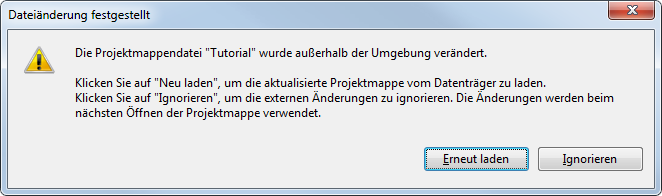
\includegraphics[scale=0.75]{figures/PNG/vs_detect_change_tutorial.png}
	\caption{\emph{Visual Studio Solution} reload prompt after \emph{CMake} has regenerated the build system.}
	\label{fig:vs_detect_change_tutorial}
\end{figure}

	\item You should now see the \verb|xme_adv_chatCalculator| item in the \emph{Project Navigator} pane in \emph{Visual Studio}.
		You can comfortably edit the source and header file of the component from there.

\begin{figure}[htpb]
	\centering
	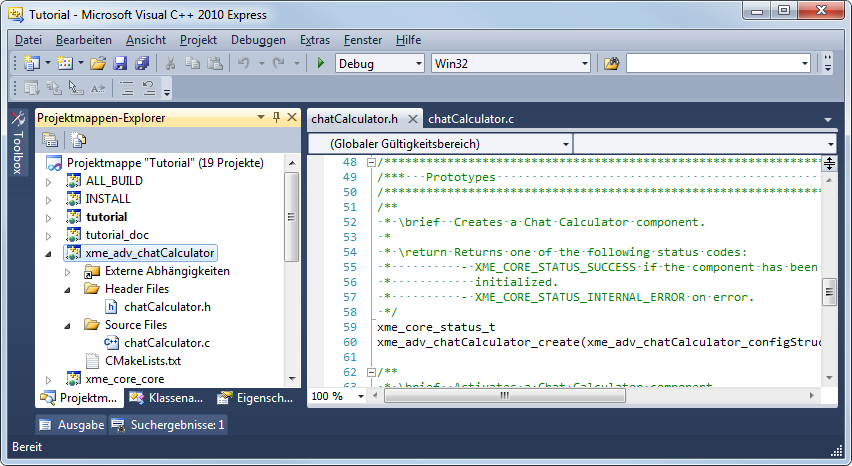
\includegraphics[width=\textwidth]{figures/PNG/vs_chatCalculator.png}
	\caption{\texttt{xme\_adv\_chatCalculator} component in the \emph{Visual Studio Project Navigator} pane.}
	\label{fig:vs_chatCalculator}
\end{figure}

	\item The component we have just added comes with some example code that we have to adapt in order to implement the \emph{Chat Calculator}.
		Open the respective files \verb|chatCalculator.h| and \verb|chatCalculator.c| found in \verb|<XME_ROOT>/xme/adv| to make yourself familiar with the generated code.
		You will notice that the generated example code publishes and subscribes the \verb|XME_CORE_TOPIC_EVENT| topic
		and that a task is created that prints a message every two seconds.
		The publication and subscription handles as well as the task handle is stored in the component's configuration structure \verb|xme_adv_chatCalculator_configStruct_t|.
		
		We can reuse the existing functionality for implementing the \emph{Chat Calculator},
		because the calculator has to listen (read: subscribe) to a specific chat room
		and print (read: publish) the result of the calculation.
		Furthermore, we need to announce the presence of the \emph{Chat Calculator} every 30~seconds,
		for which the task can be used.
		
		In order to ensure maximum flexibility (and to demonstrate how to use configuration variables),
		we will configure the topic of the chat room to enter (i.e., the topic) in \emph{Chat Calculator}'s configuration.
		For this, we will define a member variable called \verb|topic| in the comfiguration structure
		that we can set to an arbitrary value in our main program when we instantiate the component.
		In \verb|chatCalculator.h|, apply the following two changes:

\begin{lstlisting}[numbers=left,firstnumber=33]
/*************************************************************************/
/***   Type definitions                                                ***/
/*************************************************************************/
typedef struct
{
	// public
	xme_core_topic_t topic;                             /~~/ Change this line
	// private
/*	int dummyState; */                       /~~/ Comment or remove this line
	xme_core_resourceManager_taskHandle_t taskHandle;
	xme_core_dcc_publicationHandle_t publicationHandle;
	xme_core_dcc_subscriptionHandle_t subscriptionHandle;
}
xme_adv_chatCalculator_configStruct_t;
\end{lstlisting}

		We can leave the rest of the header file as-is.

	\item Now it is time to implement the actual functionality in \verb|chatCalculator.c|.
		Start by changing the published and subscribed topic to the chat room in which we want the \emph{Chat Calculator} to be.
		Apply the following four changes:

\begin{lstlisting}[numbers=left,firstnumber=69]
xme_core_status_t
xme_adv_chatCalculator_create(xme_adv_chatCalculator_configStruct_t* config)
{
	// TODO: Initialize component state
/*	config->dummyState = 0; */               /~~/ Comment or remove this line

/*	// TODO: Add code */                    /~~/ Comment or remove this block
//	XME_LOG(XME_LOG_NOTE, "Create function of Chat Calculator called!\n");

	// Example: Publish a topic
	config->publicationHandle =
		xme_core_dcc_publishTopic
		(
			config->topic,                              /~~/ Change this line
			XME_CORE_MD_EMPTY_META_DATA,
			false,
			NULL
		);

	// Check for errors
	if (XME_CORE_DCC_INVALID_PUBLICATION_HANDLE == ~\LstSuppressNumber~
		                                         config->publicationHandle) ~\LstReactivateNumber~
	{
		return XME_CORE_STATUS_INTERNAL_ERROR;
	}

	// Example: Subscribe to a topic
	config->subscriptionHandle =
		xme_core_dcc_subscribeTopic
		(
			config->topic,                              /~~/ Change this line
			XME_CORE_MD_EMPTY_META_DATA,
			false,
			_xme_adv_chatCalculator_receiveDataCallback,
			config
		); ~\LstSuppressNumber~

	[...]                           /~~/ Leave the rest of the function as-is
} ~\LstReactivateNumber~
\end{lstlisting}

	\item Now we should adapt the \verb|_xme_adv_chatCalculator_receiveDataCallback()| function,
		which handles incoming data for the subscribed topic:

\begin{lstlisting}[numbers=left,firstnumber=28]
/*************************************************************************/
/***   Implementation                                                  ***/
/*************************************************************************/
// TODO: Use or remove this sample topic subscription callback function:
static
void
_xme_adv_chatCalculator_receiveDataCallback(xme_hal_sharedPtr_t dataHandle, ~\LstSuppressNumber~
                                                            void* userData) ~\LstReactivateNumber~
{
	// TODO: In case you supply the component's configuration instance
	//       via userData when subscribing, you can access it here:
	xme_adv_chatCalculator_configStruct_t* config = ~\LstSuppressNumber~
                          (xme_adv_chatCalculator_configStruct_t*)userData; ~\LstReactivateNumber~

/*	// TODO: Add code */                    /~~/ Comment or remove this block
//	XME_LOG(XME_LOG_NOTE, "Receive data callback function called!\n");
	
/*	// Example: Print data to screen */     /~~/ Comment or remove this block
//	{
//		const char* message = xme_hal_sharedPtr_getPointer(dataHandle);
//		XME_LOG(XME_LOG_NOTE, "Received: %s\n", message);
//	}

	/~~/ Add all the following lines

	char* input = (char*)xme_hal_sharedPtr_getPointer(dataHandle);
	int size = xme_hal_sharedPtr_getSize(dataHandle);

	// Output data
	char output[512];

	// Sanitize input
	input[size-1] = 0;

	// Strip person's name
	input = strchr(input, ':');
	if (NULL == input)
	{
		// Invalid message format
		return;
	}
	input += 2;

	if (0 != strncmp(input, "!calc ", 6))
	{
		// Not a calculation command
		return;
	}

	_xme_adv_chatCalculator_getResultString
	(
		input, output, sizeof(output)
	);

	if (0 != strlen(output))
	{
		xme_core_dcc_sendTopicData
		(
			config->publicationHandle,
			(void*)output, strlen(output)+1
		);
	}
}
\end{lstlisting}

	\item Add the \verb|_xme_adv_chatCalculator_getResultString()| function, which calculates the result of an operation,
		above \verb|_xme_adv_chatCalculator_receiveDataCallback()|:

\begin{lstlisting}[numbers=left,firstnumber=31]
static
void
_xme_adv_chatCalculator_getResultString(char* in, char* out, int outSize)
{
	// Error messages
	const char* error_syntax = "The expression could not be evaluated";
	const char* error_zero = "Division by zero";
	const char* error_op = "Invalid operator";

	double operand1, operand2, result;
	char op;
	char* pos;

	// Parse string
	pos = strchr(in, 0x20);
	if (NULL == pos)
	{
		strcpy_s(out, outSize, error_syntax);
		return;
	}
	operand1 = atof(pos+1);

	pos = strchr(pos+1, 0x20);
	if (NULL == pos)
	{
		strcpy_s(out, outSize, error_syntax);
		return;
	}
	op = *(pos+1);
	
	// Ignore own announcement message
	if ('<' == op)
	{
		out[0] = 0;
		return;
	}

	pos = strchr(pos+1, 0x20);
	if (NULL == pos)
	{
		strcpy_s(out, outSize, error_syntax);
		return;
	}
	operand2 = atof(pos+1);

	// Check for operator and division by zero
	if (!_xme_adv_chatCalculator_isOperationValid(op))
	{
		strcpy_s(out, outSize, error_op);
		return;
	}
	if (_xme_adv_chatCalculator_isDivisionByZero(op, operand2))
	{
		strcpy_s(out, outSize, error_zero);
		return;
	}

	// Calculate result
	result =
		_xme_adv_chatCalculator_calculateResult(operand1, op, operand2);

	// Output result
	sprintf_s
	(
		out, outSize, "%lf %c %lf = %lf",
		operand1, op, operand2, result
	);
}
\end{lstlisting}

	\item Add the following two includes to \verb|chatCalculator.c|:
	
\begin{lstlisting}[numbers=left,firstnumber=23]
/*************************************************************************/
/***   Includes                                                        ***/
/*************************************************************************/
#include "xme/adv/chatCalculator.h"

#include <~\texttt{float}~.h>                                          /~~/ Add this line
#include <math.h>                                          /~~/ Add this line
\end{lstlisting}

	\item Add the following helper functions above \verb|_xme_adv_chatCalculator_getResultString()|:

\begin{lstlisting}[numbers=left,firstnumber=34]
static
bool
_xme_adv_chatCalculator_isOperationValid(char operation)
{
	return ('+' == operation || '-' == operation ||
		'/' == operation || '*' == operation);
}

static
bool
_xme_adv_chatCalculator_isDivisionByZero(char operation, double operand2)
{
	return ('/' == operation && abs(operand2) < DBL_EPSILON);
}

static
double
_xme_adv_chatCalculator_calculateResult(double operand1, char operation,
                                                         double operand2)
{
	if ('+' == operation)
	{
		return operand1 + operand2;
	}
	if ('-' == operation)
	{
		return operand1 - operand2;
	}
	if ('*' == operation)
	{
		return operand1 * operand2;
	}
	if ('/' == operation)
	{
		// Division by zero is handled in isDivisionByZero()
		return operand1 / operand2;
	}

	// Invalid operation is handled in isOperationValid()
	return 0;
}
\end{lstlisting}

	\item Change the text the task sends to the chat room and remove debug output:

\begin{lstlisting}[numbers=left,firstnumber=205]
// TODO: Use or remove this sample task callback function:
static
void
_xme_adv_chatCalculator_taskCallback(void* userData)
{
	// TODO: In case you supply the component's configuration instance
	//       via userData when creating the task, you can access it here:
	xme_adv_chatCalculator_configStruct_t* config = ~\LstSuppressNumber~
                          (xme_adv_chatCalculator_configStruct_t*)userData; ~\LstReactivateNumber~

/*	// TODO: Add code */                    /~~/ Comment or remove this block
//	XME_LOG(XME_LOG_NOTE, "Task callback function called!\n");

	// Example: Send data
	{                                         /~~/ Change the following lines
		static const char* message = "Chat Calculator awaiting commands.\n"
			"Usage: !calc <operand1> <operation> <operand2>"; ~\LstSuppressNumber~
		[...]                       /~~/ Leave the rest of the function as-is
	}
} ~\LstReactivateNumber~
\end{lstlisting}

	\item Configure the task to fire every 30 seconds instead of every two seconds
		and remove debug output:

\begin{lstlisting}[numbers=left,firstnumber=272]
xme_core_status_t
xme_adv_chatCalculator_activate(xme_adv_chatCalculator_configStruct_t* config)
{
/*	// TODO: Add code */                    /~~/ Comment or remove this block
//	XME_LOG(XME_LOG_NOTE, "Activate function of Chat Calculator called!\n");

	// Example: Start a task:
	config->taskHandle =
		xme_core_resourceManager_scheduleTask
		(
			1000,
			30000,                                      /~~/ Change this line
			XME_HAL_SCHED_PRIORITY_NORMAL,
			_xme_adv_chatCalculator_taskCallback,
			config
		); ~\LstSuppressNumber~

	[...]                           /~~/ Leave the rest of the function as-is
} ~\LstReactivateNumber~
\end{lstlisting}

	\item Finally, remove some more debug output:

\begin{lstlisting}[numbers=left,firstnumber=298]
void
xme_adv_chatCalculator_deactivate(xme_adv_chatCalculator_configStruct_t* config)
{
/*	// TODO: Add code */                    /~~/ Comment or remove this block
//	XME_LOG(XME_LOG_NOTE, "Deactivate function of Chat Calculator called!\n"); ~\LstSuppressNumber~

	[...]                       /~~/ Leave the rest of the function as-is
} ~\LstReactivateNumber~
\end{lstlisting}

\begin{lstlisting}[numbers=left,firstnumber=308]
void
xme_adv_chatCalculator_destroy(xme_adv_chatCalculator_configStruct_t* config)
{
/*	// TODO: Add code */                    /~~/ Comment or remove this block
//	XME_LOG(XME_LOG_NOTE, "Destroy function of Chat Calculator called!\n"); ~\LstSuppressNumber~

	[...]                       /~~/ Leave the rest of the function as-is
} ~\LstReactivateNumber~
\end{lstlisting}

	\item That's it! Compile and run the \verb|tutorial| example (press \emph{F7} and \emph{F5} in \emph{Visual Studio}).
		Test the new component by letting the \emph{Chat Calculator} do your math homework ;)
\end{enumerate}

\section{More Examples}

You might consider implementing the following components to get to know \xme even better:
\begin{itemize}
	\item A ``spammer'' component that sends unsolicited advertisements to chat channels.
	\item A component that keeps track of all persons in each chat room and supports a ``\verb|!who|'' command to print a list
		(you might want to extend the \emph{Chat Example} to publish additional data in order to do this).
	\item A ``lunch time'' component that announces lunch time at noon in every chat room.
\end{itemize}